\documentclass[11pt,a4paper]{article}
\usepackage[T1]{fontenc}
\usepackage[utf8]{inputenc}
\usepackage{lmodern,amsmath,amssymb,amsthm,mathtools}
\usepackage[a4paper,margin=25mm,headheight=15pt]{geometry}
\usepackage{microtype,booktabs,array,enumitem,xcolor,fancyhdr,needspace}
\usepackage{tikz}
\usetikzlibrary{arrows.meta,positioning,calc,fit,decorations.pathreplacing}
\usepackage[colorlinks=true,linkcolor=blue!40!black,citecolor=blue!40!black,urlcolor=blue!40!black]{hyperref}
\usepackage[nameinlink,noabbrev]{cleveref}
\definecolor{ink}{HTML}{183447}
\definecolor{accent}{HTML}{176B83}
\definecolor{pale}{HTML}{EDF4F6}
\usepackage[font=small,labelfont=bf]{caption}
\setlength{\parindent}{1.2em}
\setlength{\parskip}{2pt plus 1pt}
\setlength{\emergencystretch}{1.5em}
\setlist{nosep,leftmargin=1.7em,topsep=4pt}
\pagestyle{fancy}
\fancyhf{}
\fancyhead[L]{\small An Optimal Deterministic Adversary for Sorting}
\fancyhead[R]{\small\color{ink}Nicholas Nash}
\fancyfoot[C]{\thepage}
\renewcommand{\headrulewidth}{0.3pt}
\newtheorem{theorem}{Theorem}[section]
\newtheorem{lemma}[theorem]{Lemma}
\newtheorem{proposition}[theorem]{Proposition}
\newtheorem{corollary}[theorem]{Corollary}
\theoremstyle{definition}
\newtheorem{definition}[theorem]{Definition}
\newtheorem{remark}[theorem]{Remark}
\newcommand{\vol}{\operatorname{vol}}
\newcommand{\Prb}{\mathbb P}
\newcommand{\E}{\mathbb E}
\newcommand{\R}{\mathbb R}
\newcommand{\ceil}[1]{\left\lceil #1\right\rceil}
\newcommand{\floor}[1]{\left\lfloor #1\right\rfloor}
\newcommand{\half}{\tfrac12}
\DeclareMathOperator{\dist}{dist}
\hypersetup{pdftitle={An Optimal Deterministic Adversary for Sorting},pdfauthor={Nicholas Nash},pdfsubject={A deterministic sorting adversary with asymptotically optimal comparison lower bound}}
\title{An Optimal Deterministic Adversary for Sorting}
\author{Nicholas Nash\\[3pt]{\small\href{https://orcid.org/0009-0003-0475-7852}{ORCID: 0009-0003-0475-7852}}}
\date{8 November 2026}
\newcommand{\logtwo}{\log_2}
\begin{document}
\maketitle
\begin{abstract}
This paper describes an optimal deterministic, polynomial-time adversary for
ordinary sorting. For any correct sorting algorithm, the adversary forces that
algorithm to make $(1-o(1))n\logtwo n$ comparisons. The best previously known
adversary forced $\frac{37}{64}n\logtwo n$ comparisons.
The adversary recursively moves items into ordered subproblems, extending the
classical framework in which items move down a binary tree.
\end{abstract}

\section*{Methodological disclosure}
Except for the abstract, the text of this paper is AI-generated using
GPT 6 Astra. The author is working on a clear, human-readable exposition.

\section{Introduction}\label{sec:classical}

The information-theoretic lower bound for sorting has a simple adversarial
interpretation. Keep the set of total orders consistent with the answers
given so far, and answer each comparison so as to retain a larger half of
that set. Starting from $n!$ orders, this adversary forces at least
$\log_2(n!)$ comparisons. Its direct implementation requires counting linear
extensions of a partial order, a $\#\mathrm P$-complete
problem~\cite{brightwell}. The question is whether one can obtain the same
leading constant with an efficiently computable adversary.

We consider $n$ distinct labelled keys. A sorting algorithm chooses pairs
adaptively, and must be correct for every strict total order on the labels.
An adversary is \emph{legal} if every finite sequence of its answers is
consistent with at least one such order. It sees the requested comparisons,
but need not know the sorting algorithm that generates them.
Throughout the paper, $\log$ denotes $\log_2$, and $\ln$ the natural
logarithm. The cases $n\le1$ are immediate; we assume $n\ge2$.

\begin{theorem}\label{thm:main}
There is a deterministic legal adversary, initialized using only $n$, that
performs a fixed polynomial number of bit operations per comparison and
forces every correct comparison sorter to make
\[
(1-o(1))n\log n
\]
comparisons. The term $o(1)$ tends to zero as $n\to\infty$.
\end{theorem}

Merge sort uses at most $n\ceil{\log n}$ comparisons, so the leading
coefficient is optimal. Our construction is asymptotic: its parameter
choice establishes a uniform polynomial bound, but is not intended for
practical running times.

\subsection{From binary trees to retained comparisons}

Atallah and Kosaraju~\cite{atallah} gave an efficient sorting adversary with
leading coefficient $1/2$. Related adversaries occur in the work of
Borodin, Guibas, Lynch, and Yao~\cite{borodin} on searching after partial
sorting, Richards and Vaidya~\cite{richards} on the distribution of
comparisons among keys, and Brodal, Chaudhuri, and
Radhakrishnan~\cite{brodal} on maintaining the minimum.
The binary-tree rule of Borodin et al. and Brodal et al. provides the
starting point for our construction.

Place every item at the root of an ordered binary tree. Items in disjoint
subtrees have the left-to-right order of those subtrees. A comparison changes
the placement as follows.
\begin{itemize}
\item If both items occupy the same node, move one to its left child and
the other to its right child, and answer accordingly.
\item If one item is at an ancestor of the other, move the higher item to
the child whose subtree does not contain the lower item.
\item If their nodes are unrelated by ancestry, answer from their
left-to-right order, without moving either item.
\end{itemize}
Each comparison increases the sum of item depths by at most two.
At completion, occupied nodes must be distinct and unrelated by ancestry:
otherwise two represented items can occur in either relative order, leaving
an unresolved comparison. Their binary addresses are therefore prefix-free.
If their depths are $d_1,\ldots,d_n$, the corresponding dyadic intervals
are disjoint, giving
\[
\sum_i2^{-d_i}\le1,
\qquad
2^{-\frac1n\sum_i d_i}\le\frac1n\sum_i2^{-d_i}\le\frac1n.
\]
Convexity gives the bound on $2^{-\frac1n\sum_i d_i}$. Hence $\sum_i d_i\ge n\log n$, and
at least $\tfrac12 n\log n$ comparisons are
necessary~\cite[Section~4.1]{brodal}.

The tree makes the state easy to maintain, but commits to some relations
that have never been queried. After answers $A<B$ and $C<D$ at the same
node, for example, it may place $A,C$ in the left child and $B,D$ in the
right. This also fixes $A<D$ and $C<B$. Figure~\ref{fig:retained}
contrasts this separation with retaining just the two inequalities.

\begin{figure}[tb]
\centering
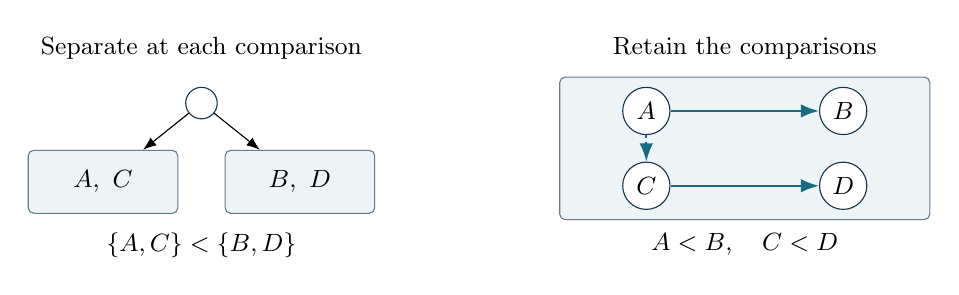
\begin{tikzpicture}[>=Latex,font=\small,
  group/.style={draw=ink!65,rounded corners=2pt,fill=pale,minimum height=8mm},
  item/.style={circle,draw=ink,fill=white,minimum size=6mm,inner sep=1pt}]
\begin{scope}[shift={(-3.5,0)}]
\node at (0,1.15) {Separate at each comparison};
\node[circle,draw=ink,fill=white,minimum size=4mm] (root) at (0,.45) {};
\node[group,minimum width=19mm] (left) at (-1.25,-.55) {$A,\ C$};
\node[group,minimum width=19mm] (right) at (1.25,-.55) {$B,\ D$};
\draw[->] (root)--(left);
\draw[->] (root)--(right);
\node at (0,-1.35) {$\{A,C\}<\{B,D\}$};
\end{scope}
\begin{scope}[shift={(3.4,0)}]
\node at (0,1.15) {Retain the comparisons};
\draw[group] (-2.35,-1.03) rectangle (2.35,.78);
\node[item] (a) at (-1.25,.35) {$A$};
\node[item] (b) at (1.25,.35) {$B$};
\node[item] (c) at (-1.25,-.6) {$C$};
\node[item] (d) at (1.25,-.6) {$D$};
\draw[->,thick,accent] (a)--(b);
\draw[->,thick,accent] (c)--(d);
\draw[->,dash pattern=on 1pt off 1.5pt,thick,accent] (a)--(c);
\node at (0,-1.35) {$A<B,\quad C<D$};
\end{scope}
\end{tikzpicture}
\caption{Two answered comparisons need not determine all cross-relations.
The binary-tree rule separates the pairs spatially. A group with stored
arrows retains the freedom to answer later cross-comparisons. The dashed
arrow shows how a subsequent answer $A<C$ can be stored in the same group.}
\label{fig:retained}
\end{figure}

Kaplan, Zamir, and Zwick~\cite{kzz} improved the leading coefficient to
$37/64$ by retaining more structure before moving items down the tree.
Their constructions allow ordered pairs within a node, together with rules
for resolving interactions between these pairs. The present adversary
extends this approach: a node retains a directed graph of comparisons, and
an item moves to a child only when the graph must be simplified or its
coordinate must be prepared for a query.

\subsection{The construction and its analysis}

For a partial order $P$, the region of unit coordinates satisfying its
inequalities has volume $e(P)/n!$, where $e(P)$ is the number of linear
extensions: every coordinate order occupies volume $1/n!$~\cite{stanley}.
Thus retaining a larger-volume side would implement the ideal adversary
if we kept all items at the root and never simplified its constraints.

In our representation each group has auxiliary real positions in $(0,1)$,
constrained by its stored comparisons. An arrow $x\to y$ means $X_x<X_y$. The adversary chooses
an approximately larger-volume answer, retaining at least $1/2-\eta$ of
the group's feasible volume. Bounded degree and bounded directed-path
length allow this probability to be estimated from a neighborhood whose
size depends only on an accuracy parameter. The group itself may contain
arbitrarily many items.

To simplify a group, fix an item's position at an interior point $c$, replace
its incident arrows by interval bounds, and give it a fresh coordinate in
a child at $c$. This preserves every answered comparison. If $f_x(c)$ is
the density of the fixed coordinate, the product $Z$ of all group volumes
is multiplied by exactly $f_x(c)$. A well-chosen position can therefore
recover volume while removing constraints from the graph.

The proof assigns a small interval to each child and embeds the entire
recursive state in the unit cube. The widths of these intervals contribute
a factor $\mathcal W$. Initially $n!Z\mathcal W=n!$; when a sorter finishes,
the embedding lies in one order region and $n!Z\mathcal W\le2^n$.
We then use the potential
\[
\Psi=n!Z^\beta\mathcal W\,2^{-\tau e},
\]
where $e$ is the number of stored arrows, $\beta=1+o(1)$, and $\tau=o(1)$.
The extra volume factor and the charge for stored arrows make every complete
repair nondecreasing in $\Psi$. Each comparison reduces $\log\Psi$ by at
most $1+o(1)$, giving the theorem.

Section~\ref{sec:algorithm} specifies the algorithm before its analysis.
Sections~\ref{sec:legal} and~\ref{sec:oracle} establish legality and the
local numerical guarantees. Sections~\ref{sec:accounting}
and~\ref{sec:potential} give the packing and potential arguments, and
Section~\ref{sec:runtime} proves the uniform polynomial bound.
The proofs of the density bounds, locality, and exact local volume calculation
appear in the appendices. The manuscript source is available online.\footnote{\url{https://github.com/nicknash/sorting-adversary-proofs/tree/main/for-humans}}

\section{The adversary}\label{sec:algorithm}

The adversary maintains a rooted tree of groups. A group records comparisons
among items whose relative order is still being resolved there. An item may
leave a group by fixing its position and continuing in a child at that
position. We call this operation a \emph{refinement}.

Fix an integer $k\ge16$. The algorithm uses the parameters
\begin{equation}\label{eq:parameters}
\eta=\frac1{100k},\qquad H=2^{2k},\qquad
B=(k+1)^{2H+1},\qquad R=2^{2kB}.
\end{equation}
Between comparison calls, the graph in each group has degree less than $k$
and no directed path on $H$ vertices. These two restrictions will make the
probability calculations local. The threshold $1/R$ determines when a queried
coordinate must first be refined. Section~\ref{sec:runtime} selects $k$ as a
function of $n$; for now it is fixed.

\subsection{The state of a group}

At each node $v$, every item represented there is either \emph{free} or belongs
to a child subtree. A free item $x$ has an auxiliary coordinate $X_x$ in an open
interval $(a_x,b_x)\subseteq(0,1)$. These coordinates describe possible orders;
they are not the unknown key values. A directed acyclic graph on the free
items stores inequalities $X_x<X_y$. Each child has a fixed position
$c\in(0,1)$, its \emph{anchor}, and its own copy of the unit interval.
Different children of one node have different anchors.

Each original item has exactly one free coordinate in the entire tree. At
every ancestor of its node it is represented by the anchor of the child
containing it. Initially all $n$ items are free at the root, their intervals
are $(0,1)$, and there are no arrows or children.

The feasible region of a node is
\begin{equation}\label{eq:node-region}
K_v=\{X:a_x<X_x<b_x\text{ for all free }x,
             \quad X_x<X_y\text{ for every arrow }x\to y\}.
\end{equation}
Write $V_v=\vol(K_v)$, with volume one when the node has no free items, and
define
\begin{equation}\label{eq:Z}
Z=\prod_v V_v.
\end{equation}
Thus $Z=1$ initially. We shall prove that every reached state satisfies
$0<Z\le1$. The algorithm never
calculates this product. It calculates probabilities only in small induced
subgraphs, as specified in Section~\ref{sec:oracle}.

Only actual comparisons create arrows. The graph is simple: repeated
comparisons do not create parallel arrows, and transitive consequences are
not inserted. The number of stored arrows will matter in the proof.

We maintain all interval bounds implied by the arrows. Write $y\preceq x$
if $y=x$ or a directed path leads from $y$ to $x$. The \emph{effective interval}
of $x$ is $(\ell_x,r_x)$, where
\begin{equation}\label{eq:effective}
\ell_x=\max_{y\preceq x}a_y,\qquad
r_x=\min_{y\succeq x}b_y,\qquad W_x=r_x-\ell_x.
\end{equation}
The operation \textnormal{\textsc{Tighten}} replaces every stored interval by its effective
interval. It is performed after every change to an interval or arrow, before
testing widths or calculating probabilities. The resulting bounds remain
stored when arrows are later removed. A coordinate is \emph{wide} if
$W_x\ge1/R$, and \emph{narrow} otherwise.

\subsection{Choosing an answer}

To compare original items $A$ and $B$, descend while both belong to the same
child. At the first node where their representations differ, each is either
a free coordinate or a child anchor. Two different anchors determine the
answer. Otherwise at least one representation is free.

Suppose first that both are free. Under the uniform volume measure on $K_v$,
let
\[
p=\Prb(X_A<X_B)=\frac{\vol(K_v\cap\{X_A<X_B\})}{V_v}.
\]
The probability notation is only a ratio of volumes; the adversary makes no
random choices. Given an estimate $\widehat p$ with
$|\widehat p-p|\le\eta$, it answers $A<B$ if $\widehat p\ge1/2$, and $B<A$
otherwise. Since equality has volume zero, the chosen answer retains at
least $1/2-\eta$ of $V_v$. It is stored as an arrow. For a free coordinate
and an anchor $c$, write $x$ for the free item and use $\Prb(X_x<c)$.
Store the resulting upper or lower interval bound, reversing the reported
label order when the free item is $B$.

The local estimator requires a wide coordinate for a threshold query, and
at least one wide endpoint for a two-coordinate query. If this condition
fails, the adversary refines a queried item before answering.

\subsection{Choosing an anchor and refining an item}

Every anchor is the midpoint of a dyadic cell:
\begin{equation}\label{eq:dyadic}
c=(j+\tfrac12)2^{-m},\qquad 0\le j<2^m,\quad m\ge0.
\end{equation}
We call $m$ its \emph{address length}: $m$ binary digits specify the cell.
The reduced denominator of $c$ is $2^{m+1}$, so its position determines
$m$ uniquely. Reusing an anchor therefore also reuses its address length.

There are two rules for choosing $c$.

\begin{enumerate}
\item For a wide item, start with the cell $[0,1]$. At its midpoint $c$,
estimate $F_x(c)=\Prb(X_x<c)$ to error at most $\eta$.
If the estimate is below $1/4$, retain the right half; if it is above $3/4$,
retain the left half; otherwise accept $c$. Repeat within the retained cell.
\item For a narrow item, choose the dyadic length $b=2^{-m}$ satisfying
$W_x/8<b\le W_x/4$. Choose the midpoint of a cell of this length nearest
to $(\ell_x+r_x)/2$, taking the smaller midpoint in case of a tie.
\end{enumerate}

Both choices lie strictly inside the effective interval. Their density
guarantees are proved in Section~\ref{sec:oracle}.

To refine $x$ at $c$, fix $X_x=c$, remove $x$ from the parent's free graph,
and replace each incident arrow by the corresponding bound on its other
endpoint. Thus $y\to x$ becomes $X_y<c$, and $x\to z$ becomes $X_z>c$.
Retain all other stored bounds and tighten the parent. Then admit $x$ to
the child at $c$, creating the child if necessary, as an isolated coordinate
with interval $(0,1)$. The child's previous data stay unchanged.

\begin{figure}[tb]
\centering
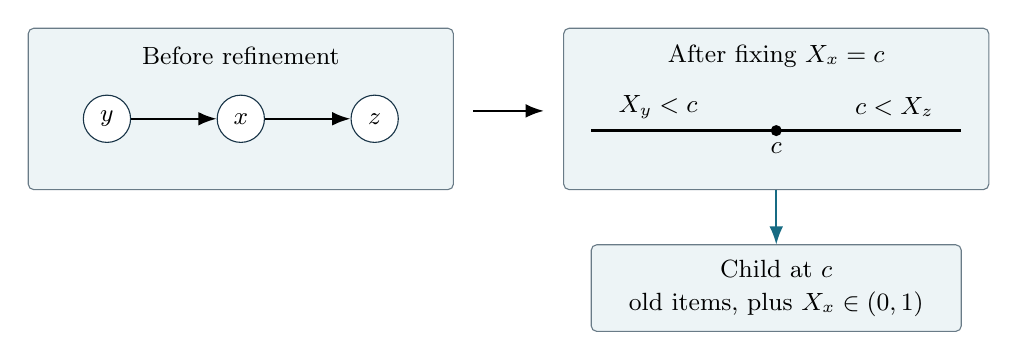
\begin{tikzpicture}[>=Latex,font=\small,
  item/.style={circle,draw=ink,fill=white,minimum size=6mm,inner sep=1pt},
  group/.style={draw=ink!65,rounded corners=2pt,fill=pale}]
\begin{scope}[shift={(-3.4,0)}]
\draw[group] (-2.7,-.9) rectangle (2.7,1.15);
\node at (0,.8) {Before refinement};
\node[item] (y) at (-1.7,0) {$y$};
\node[item] (x) at (0,0) {$x$};
\node[item] (z) at (1.7,0) {$z$};
\draw[->,thick] (y)--(x);
\draw[->,thick] (x)--(z);
\end{scope}
\draw[->,thick] (-.45,.1)--(.45,.1);
\begin{scope}[shift={(3.4,0)}]
\draw[group] (-2.7,-.9) rectangle (2.7,1.15);
\node at (0,.8) {After fixing $X_x=c$};
\draw[thick] (-2.35,-.15)--(2.35,-.15);
\fill (0,-.15) circle (2pt);
\node[below] at (0,-.18) {$c$};
\node at (-1.5,.15) {$X_y<c$};
\node at (1.5,.15) {$c<X_z$};
\draw[group] (-2.35,-2.7) rectangle (2.35,-1.6);
\node at (0,-1.9) {Child at $c$};
\node at (0,-2.35) {old items, plus $X_x\in(0,1)$};
\draw[->,thick,accent] (0,-.9)--(0,-1.6);
\end{scope}
\end{tikzpicture}
\caption{A refinement preserves the comparisons incident to $x$ as interval
bounds in the parent. The relative order of $x$ and the items already at the
same anchor is resolved inside the child.}
\label{fig:refinement}
\end{figure}

\subsection{The complete comparison procedure}

The following procedures specify all state changes. Ties between eligible
items are resolved by label order. A path is selected by the lexicographically
first eligible label sequence. Degree counts neighbors without regard to
edge direction; path length below counts vertices.

\begin{quote}
\textbf{Restore$(v)$.}
\begin{enumerate}
\item While the free graph of $v$ has a vertex of degree at least $k$,
refine such a vertex.
\item While it contains a directed path on $H$ vertices, select one such
path and refine all its vertices in label order. Complete this entire list
before selecting another path.
\end{enumerate}
\end{quote}

\begin{quote}
\begin{minipage}{\linewidth}
\textbf{Compare$(A,B)$.}
\begin{enumerate}
\item Descend through common children to the first node $v$ where the
representations differ. If both are anchors, return their order.
\item Tighten $v$. If none of the free queried coordinates is wide,
refine one of them and restart step 1.
\item Estimate the probability of $A<B$ to additive error $\eta$ and select
an answer by the rule above. Store its arrow or interval bound.
\item Tighten $v$, run \textnormal{\textsc{Restore}}$(v)$, and return the selected answer.
\end{enumerate}
\end{minipage}
\end{quote}

Every answer is also entered in a separate comparison graph on the original
labels, before restoration or, for an anchor answer, before returning.
This graph records the public transcript. Its edges do not count toward the
degree restrictions or the active arrow count used below. It will supply a
compatible total order for the finite stopping rule in
Section~\ref{sec:runtime}.

\section{Refinement and its guarantees}\label{sec:legal}

We now prove the refinement guarantees used in Section~\ref{sec:potential}:
moving an item preserves the answers already given, and the resulting
change in volume controls the cost of choosing a child.

\subsection{Preserving the represented orders}

We use the interpretation of the state given in Section~\ref{sec:overview}.
Assignments with equal free coordinates, or with a free coordinate equal
to an anchor, lie on a finite union of sets of volume zero and are excluded
when reading an order. We maintain the following invariant:
\begin{quote}
Every represented total order respects every comparison already answered.
\end{quote}
The state may discard some orders that still respect the answers. Legality
requires only that at least one remains. Positive volume in every node
will ensure this.

The invariant must continue to hold when refinement removes an arc from
an in-node DAG.

\begin{lemma}[Effective intervals and sections]\label{lem:interior}
Replacing interval bounds by their effective endpoints leaves the
feasible region unchanged.
The region has positive volume if and only if every effective width is
positive. When these widths are positive, fixing $X_x=c$ at any
$c\in(\ell_x,r_x)$ leaves a
positive-volume section in the remaining coordinates.
\end{lemma}
\begin{proof}
If $y\ne x$ precedes $x$ on a directed path, every feasible assignment
satisfies $X_x>X_y>a_y$; the stored bound $X_x>a_x$ covers $y=x$.
Taking the maximum over these bounds gives $X_x>\ell_x$. The upper-bound argument is the reverse. Thus all bounds
given by \eqref{eq:effective} already hold.

Positive volume requires positive widths. Conversely, suppose all widths
are positive. Along an arc $x\to y$, the definitions give
$\ell_x\le\ell_y$ and $r_x\le r_y$. Choose numbers $0<\theta_x<1$
increasing in a topological order, and set
\[
X_x=(1-\theta_x)\ell_x+\theta_xr_x.
\]
Increasing $\theta_x$ to $\theta_y$ strictly increases this value because
$r_x>\ell_x$. Replacing its endpoints by the larger endpoints
$\ell_y,r_y$ cannot decrease it. Hence $X_x<X_y$. All coordinates are
inside their intervals and all arc inequalities hold strictly, so a
sufficiently small open neighborhood of this assignment is feasible.

Now fix $X_x=c$ and delete its coordinate. The inequalities imposed by
its incident arcs become upper bounds $c$ at its in-neighbors and lower
bounds $c$ at its out-neighbors. Upper bounds propagate only backward
along arcs, and lower bounds only forward. Any lower bound that previously
reached a successor through $x$ is superseded by $c>\ell_x$; any upper
bound that reached a predecessor through $x$ is superseded by $c<r_x$.
Thus the new effective intervals are
\[
\begin{cases}
(\ell_y,\min(r_y,c)),&y\text{ precedes }x,\\
(\max(\ell_y,c),r_y),&y\text{ succeeds }x,\\
(\ell_y,r_y),&y\text{ is incomparable with }x.
\end{cases}
\]
The first two cases are disjoint because the in-node DAG is acyclic. A predecessor
retains positive width: $r_y>\ell_y$ and
$c>\ell_x\ge\ell_y$. A successor does too: $r_y>\ell_y$ and
$c<r_x\le r_y$. All other widths stay positive. The criterion just proved,
applied to the remaining in-node DAG, shows that the section has positive volume.
\end{proof}

\begin{lemma}[Refinement and child admission]\label{lem:admission}
Suppose the node regions have positive volume and the order invariant holds.
Refining $x$ at an interior anchor $c$ preserves both properties, including
when the child at $c$ already exists. The transcript implies no
relation between $x$ and any label already in that child subtree.
\end{lemma}
\begin{proof}
Consider first an existing child at $c$, and denote its label set by $S$.
Choose a feasible assignment in the parent section $X_x=c$, with the other
free coordinates pairwise distinct and different from every child anchor.
Such an assignment exists by Lemma~\ref{lem:interior}. Also choose feasible
assignments in the other nodes.

There is a positive distance from $c$ to every other child anchor and
every free parent coordinate in this assignment. All incident inequalities at $x$ are strict. Thus, with
everything else fixed, $x$ can be moved slightly to either side of $c$
while keeping the old state feasible. The resulting two represented orders
place $x$ immediately before or immediately after the entire block $S$.
Both orders respect the transcript. For each $y\in S$, one has $x<y$ and
the other has $y<x$; neither relation can therefore be implied by the
transcript.

Now take any order represented after the refinement. Deleting $x$ from the
child leaves an assignment of its old coordinates and hence an old child
order. Apply the preceding perturbation using this assignment's parent
coordinates and old child coordinates. It gives two feasible old orders
that agree with the new one on every label except $x$. The new order
inserts $x$ somewhere into their child block. No
answered comparison joins $x$ to a label in $S$, so this insertion violates
none of them. Relative to every label outside $S\cup\{x\}$, the whole
block occupies the old anchor position. The item $x$ is consequently on
the same side of each outside label as in either of the two feasible old
orders above. Comparisons between other labels are unchanged. The new
order therefore respects the entire transcript.

If there was no child at $c$, the same argument uses an empty block: the
new singleton child places $x$ where its fixed parent coordinate stood.
Finally, the remaining parent region is a positive-volume section, and
the child receives an independent coordinate in $(0,1)$. All node regions
remain positive.
\end{proof}

\subsection{The volume gained by refinement}\label{sec:refinement-volume}

Refining an item $x$ stored at node $v$ fixes $X_x=c$ in $v$ and gives
$x$ a fresh unit coordinate in the child. To measure the volume change, let
$S_x(c)$ be the volume of the section of $K_v$ obtained by fixing
$X_x=c$, measured in the remaining coordinates. Under the uniform
distribution on $K_v$, the coordinate $X_x$ has density
\[
f_x(c)=\frac{S_x(c)}{V_v},\qquad
\Prb(a<X_x<b)=\int_a^b f_x(t)\,dt.
\]

\begin{lemma}[Refinement identity]\label{lem:section-volume}
Suppose every node region has positive volume. Refining $x$ at an interior
anchor $c$ satisfies
\begin{equation}\label{eq:refine}
\frac{Z_{\rm after}}{Z_{\rm before}}=f_x(c).
\end{equation}
\end{lemma}
\begin{proof}
Let $u$ be the child at $c$, taking $V_u=1$ if it is newly created. The
parent loses the coordinate $X_x$ and retains precisely the section of
volume $S_x(c)$. The child gains a new coordinate $U_x\in(0,1)$, with no
constraints involving its old coordinates. Its region becomes
$K_u\times(0,1)$ and still has volume $V_u$. Therefore the affected
factors in the product change as follows:
\[
V_vV_u\quad\longrightarrow\quad S_x(c)V_u.
\]
Their ratio is $S_x(c)/V_v=f_x(c)$. All other node factors stay unchanged.
The dimension lost in the parent is restored by the new child coordinate.
\end{proof}

Thus the refinement's volume gain is $g=\log f_x(c)$.

For example, the parent region $0<X_A<X_B<1$ has area $1/2$. Fixing
$X_A=1/4$ leaves the interval $X_B\in(1/4,1)$ of length $3/4$. The new
child coordinate $U_A\in(0,1)$ turns this into a rectangle of area $3/4$,
so refinement multiplies $Z$ by $3/2$; see Figure~\ref{fig:section-volume}.
Both regions represent the order $A<B$. Replacing the fixed parent
coordinate by a fresh child coordinate gives the larger area.

\begin{figure}[tb]
\centering
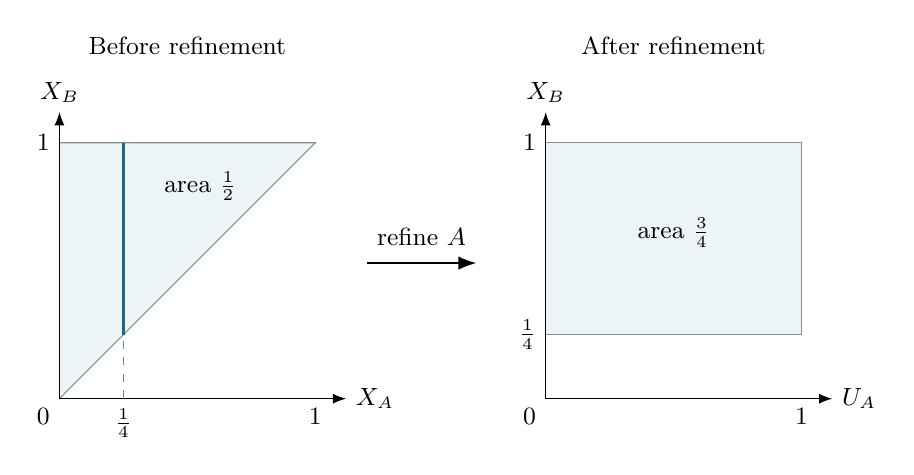
\begin{tikzpicture}[x=3.25cm,y=3.25cm,>=Latex,font=\small]
\begin{scope}
\node at (.5,1.38) {Before refinement};
\fill[pale] (0,0)--(0,1)--(1,1)--cycle;
\draw[ink!55] (0,0)--(1,1)--(0,1);
\draw[->] (0,0)--(1.12,0) node[right] {$X_A$};
\draw[->] (0,0)--(0,1.12) node[above] {$X_B$};
\draw[dashed,ink!60] (.25,0)--(.25,.25);
\draw[accent,very thick] (.25,.25)--(.25,1);
\node[below] at (.25,0) {$\frac14$};
\node[below left] at (0,0) {$0$};
\node[below] at (1,0) {$1$};
\node[left] at (0,1) {$1$};
\node at (.55,.83) {area $\frac12$};
\end{scope}
\draw[->,thick] (1.2,.53)--(1.63,.53);
\node[above] at (1.415,.56) {refine $A$};
\begin{scope}[shift={(1.9,0)}]
\node at (.5,1.38) {After refinement};
\fill[pale] (0,.25) rectangle (1,1);
\draw[ink!55] (0,.25)--(1,.25)--(1,1)--(0,1);
\draw[->] (0,0)--(1.12,0) node[right] {$U_A$};
\draw[->] (0,0)--(0,1.12) node[above] {$X_B$};
\node[below left] at (0,0) {$0$};
\node[left] at (0,.25) {$\frac14$};
\node[below] at (1,0) {$1$};
\node[left] at (0,1) {$1$};
\node at (.5,.65) {area $\frac34$};
\end{scope}
\end{tikzpicture}
\caption{The highlighted section of the triangle has length $3/4$.
Replacing the fixed parent coordinate by a fresh unit coordinate in the
child gives the rectangle on the right. Its area is $3/2$ times the
original area.}
\label{fig:section-volume}
\end{figure}

\subsection{Choosing an anchor}\label{sec:median-search}\label{sec:anchor-contract}

The choice of anchor balances two quantities: a larger density gives
more volume gain, while a smaller anchor depth costs less in
\eqref{eq:anchor-cost}. We will bound the density using the number of
coordinates comparable with $x$. Put
\begin{equation}\label{eq:comparable-bound}
B=(k+1)^{2H+1}.
\end{equation}
In an in-node DAG of degree at most $k$ and directed paths of at most
$2H$ vertices, every coordinate comparable with $x$ lies within undirected
distance $2H$ of $x$. Thus $B$ bounds the number of other coordinates
comparable with $x$.

Set the calibration width
\begin{equation}\label{eq:width-threshold}
w_*=2^{-2kB}.
\end{equation}
The finite calculations use this scale to guarantee success when a
queried coordinate has a sufficiently large effective interval.

\begin{lemma}[When certification succeeds]\label{lem:certificate-success}
Suppose a node has positive feasible volume, its in-node DAG has degree
at most $k$, and its directed paths have at most $2H$ vertices.
If any free coordinate involved in a comparison has effective width at
least $w_*$, comparison certification succeeds. If $W_x\ge w_*$, then
\textnormal{\texttt{CentralInterval}}$(v,x)$ succeeds.
\end{lemma}

Section~\ref{sec:oracle} proves this lemma. In particular, failure of a
central-interval certificate implies $W_x<w_*$. This is the information
used to justify the anchor routine's fallback.

\begin{lemma}[Anchor selection]\label{lem:anchor-density}
Suppose a node's feasible region has positive volume, its interval
endpoints are dyadic, and its in-node DAG has degree at most $k$ and
directed paths of at most $2H$ vertices. With calibration width \eqref{eq:width-threshold},
\textnormal{\texttt{ChooseAnchor}} deterministically returns an anchor
$c\in(\ell_x,r_x)$ at depth $m$ in the implicit anchor tree satisfying
\begin{equation}\label{eq:tariff}
\log f_x(c)\ge(1-1/k)m-4.
\end{equation}
If $x$ is refined because comparison certification failed, then
\begin{equation}\label{eq:failure-gain}
\log f_x(c)>k.
\end{equation}
\end{lemma}

Algorithm~\ref{alg:choose-anchor} first tries \texttt{CentralInterval}.
On success, it uses the returned interval; on failure, it uses the middle
half of the effective interval. It then selects the shallowest anchor in
the chosen interval. Both choices give the density bound required by
Lemma~\ref{lem:anchor-density}.

\begin{algorithm}[H]
\caption{\texttt{ChooseAnchor}$(x)$: choose a position for refinement.}
\label{alg:choose-anchor}
\DontPrintSemicolon
\KwIn{A free item $x$ stored at node $v$ and its effective interval $(\ell_x,r_x)$.}
\KwOut{A dyadic anchor $c\in(\ell_x,r_x)$.}
$J\gets$ \texttt{CentralInterval}$(v,x)$\;
\If{$J$ is \textnormal{\texttt{FAIL}}}{
  $W_x\gets r_x-\ell_x$\;
  $J\gets[\ell_x+W_x/4,\ r_x-W_x/4]$\;
}
$[a,b]\gets J$\;
$u\gets$ the root of the implicit anchor tree\;
\While{true}{
  \uIf{$c(u)<a$}{$u\gets$ the right child of $u$\;}
  \uElseIf{$c(u)>b$}{$u\gets$ the left child of $u$\;}
  \Else{\Return $c(u)$\;}
}
\end{algorithm}

An anchor at depth $m$ has $m+1$ fractional binary digits in reduced
form. Thus the walk finds the shortest binary fraction in $[a,b]$.

\begin{lemma}[Shortest anchor in an interval]\label{lem:shortest-anchor}
For a nondegenerate closed interval $[a,b]\subset(0,1)$, the walk in
Algorithm~\ref{alg:choose-anchor} returns its unique minimum-depth anchor.
If its node is $u$ and its depth is $m$, then
$[a,b]\subseteq I(u)$ and $|I(u)|=2^{-m}$.
\end{lemma}
\begin{proof}
Initially $[a,b]\subseteq I(u)=[0,1]$. Whenever $c(u)<a$, the whole
interval lies in the right child's interval; whenever $c(u)>b$, it lies
in the left child's interval. The rejected anchor and the other subtree
contain no candidate in $[a,b]$. The first accepted anchor therefore has
minimum depth, and every other anchor of that depth lies outside $I(u)$.
The intervals halve at every step and continue to contain $[a,b]$, so
the walk must accept before their length becomes smaller than $b-a$.
\end{proof}

\subsubsection{Density bounds for central intervals}

The first bounds use the effective width and the number of comparable
coordinates.

\begin{lemma}[Coordinate density bounds]\label{lem:fiber}
Suppose a node's feasible region has positive volume, and $x$ has at most
$B$ other comparable coordinates and effective interval $(\ell,r)$ of
width $W$. Its density satisfies
\begin{align}
f_x(t)&\le\frac{B+1}{W},\label{eq:fiber-upper}\\
f_x(t)&\ge\frac{4^{-B}}{W}
\qquad(\ell+W/4\le t\le r-W/4).\label{eq:fiber-lower}
\end{align}
\end{lemma}

The lower bound controls the fallback choice in the middle half of the
effective interval. The upper bound will help bound the probability of
an unresolved comparison. Appendix~\ref{app:geometry} proves both by
comparing convex sections.

For a certified central interval we use another consequence of convexity. A density is
\emph{log-concave} if its positive support is convex and its logarithm
is concave there. The uniform density on a convex feasible region is
log-concave, and Pr\'ekopa's marginal theorem gives the same property to
each coordinate density \cite[Theorem~8]{prekopa}. The following bound says
that a position with substantial probability on each side has density
comparable to the largest value.

\begin{lemma}[Density at central positions]\label{lem:central-quantiles}
Let $X$ have a log-concave density $f$. If
$\Prb(X\le c)\ge p$ and $\Prb(X\ge c)\ge p$ for some $0<p\le1/2$, then
\[
f(c)\ge p\sup_t f(t).
\]
\end{lemma}

Appendix~\ref{app:geometry} proves the lemma directly from log-concavity.

\subsubsection{Anchors from a certified interval}

\begin{lemma}[Certified anchor choices]\label{lem:median-search}
If \textnormal{\texttt{CentralInterval}} succeeds, the anchor $c$ selected
by Algorithm~\ref{alg:choose-anchor} has depth $m$ and satisfies
\[
\log f_x(c)\ge m-4,\qquad
\log f_x(c)\ge\log(1/W_x)-2.
\]
\end{lemma}
\begin{proof}
Let $J$ be the interval returned by \texttt{CentralInterval}, and put
$M=\sup_t f_x(t)$. By Lemma~\ref{lem:central-interval}, $J$ is contained
in $(\ell_x,r_x)$ and has probability at least $1/4$, so $M|J|\ge1/4$.
Every position $c\in J$ also has probability at least $1/4$ on each side.
Lemma~\ref{lem:central-quantiles} therefore gives $f_x(c)\ge M/4$
throughout $J$.

Lemma~\ref{lem:shortest-anchor} selects $c\in J$ at a node $u$ whose
interval contains $J$. Its interval has length $2^{-m}$, so
\[
2^{-m}f_x(c)\ge |J|\frac M4\ge\frac1{16}.
\]
This proves the first bound. Since $f_x$ integrates to one over an
interval of width $W_x$, its supremum satisfies $M\ge1/W_x$.
The inequality $f_x(c)\ge M/4$ proves the second bound.
\end{proof}

\subsubsection{The anchor guarantee}\label{sec:anchor-guarantee}

The certified choice already gives the required bound. For the fallback,
failure of the central-interval calculation implies $W_x<w_*$, so
$\log(1/W_x)>2kB$. This pays for the loss of $2B$ in the lower density
bound \eqref{eq:fiber-lower}.

\begin{proof}[Proof of Lemma~\ref{lem:anchor-density}]
The in-node DAG bounds imply that $x$ has at most $B$ other comparable
coordinates, by \eqref{eq:comparable-bound}. If central certification
succeeds, Lemma~\ref{lem:median-search} gives the stronger lower bound
$m-4$. Otherwise, Lemma~\ref{lem:certificate-success} gives
$W_x<w_*$. Write $L=\log(1/W_x)>2kB$. The fallback anchor is in the
central half of its effective interval, so \eqref{eq:fiber-lower}
gives
\[
\log f_x(c)\ge L-2B.
\]
By Lemma~\ref{lem:shortest-anchor}, its node interval contains that central
half. Hence $W_x/2\le2^{-m}$ and $m\le L+1$, giving
\[
\log f_x(c)\ge L-2B>(1-1/k)L
\ge(1-1/k)(m-1)>(1-1/k)m-4.
\]
This proves \eqref{eq:tariff} in both branches.

Now suppose comparison certification failed and the algorithm selected
$x$ for refinement. Lemma~\ref{lem:certificate-success} implies
$W_x<w_*$, regardless of the subsequent central-interval result.
If central certification succeeds, Lemma~\ref{lem:median-search} gives
\[
\log f_x(c)\ge\log(1/W_x)-2>2kB-2>k.
\]
If it fails, the fallback bound above gives
$\log f_x(c)\ge\log(1/W_x)-2B>2B(k-1)>k$.
This proves \eqref{eq:failure-gain}.
Both cases use a finite deterministic calculation to obtain the central
interval, followed by the finite walk of Lemma~\ref{lem:shortest-anchor}.
\end{proof}

\subsection{Bounds during a comparison call}\label{sec:repairs}

The preparation loop in Algorithm~\ref{alg:compare} simplifies the current
node before an answer is selected. We check that the in-node DAG bounds
hold throughout the call, and that the loop makes only finitely many
moves.

\begin{lemma}[In-node DAG bounds and termination]\label{lem:restoration}
Suppose every node region has positive volume and every in-node DAG has
degree at most $k$ and directed paths of fewer than $2H$ vertices at the
start of a call. These properties hold throughout the call. Each label
is refined at most once, so the call makes at most $n$ refinements.
\end{lemma}
\begin{proof}
A refinement uses an interior anchor by Lemma~\ref{lem:anchor-density}.
It leaves a positive-volume parent section by Lemma~\ref{lem:interior}
and gives the child a fresh unit coordinate. It deletes a vertex and its
incident arcs from the parent and adds an isolated vertex to the child,
so it cannot increase any degree or extend any directed path.

A returned comparison certificate gives its chosen answer positive
probability, so recording it preserves positive feasible volume.
Its arc cannot create a directed cycle, which would make the region
empty. Immediately before a new answer is selected,
the current in-node DAG has no path on $H$ vertices and the queried free
vertices have degree below $k$. Adding their comparison arc leaves degree
at most $k$. Any new directed path consists of two old paths joined by
this arc, so it has fewer than $2H$ vertices. An answer involving an anchor
adds only an interval bound. These observations prove positivity and
the in-node DAG bounds by induction through the call.

Once a label is refined, it has an isolated coordinate with interval
$(0,1)$ in its child. Until the final answer, every subsequent state change
is another refinement. These moves affect interval bounds only at
neighbors of the vertex being removed, so they cannot narrow this isolated
coordinate or give it an incident arc. It cannot lie on a selected path
or have degree $k$. Lemma~\ref{lem:estimation} guarantees that comparison
certification succeeds whenever such a unit-interval coordinate is
queried, so it cannot be selected after a failed certificate either.
Thus no label is selected again, even if the query is rerouted to its new
node. Every restart refines at least one label, giving the bound of $n$
refinements.
\end{proof}

\begin{proof}[Proof of Proposition~\ref{prop:legality}]
Initially every node region has positive volume, every order is represented,
and the in-node DAG bounds hold. We induct over the changes made by a
comparison call. The bounds follow from Lemma~\ref{lem:restoration}.
At a refinement, Lemma~\ref{lem:anchor-density} supplies an interior
anchor, and Lemma~\ref{lem:admission} preserves positive volume and the
order invariant. This applies to every item of a selected path, including
those whose incident arcs have already been removed by earlier moves.

If the queried labels lie in different child subtrees, their anchors
determine the answer in every represented order. Otherwise, a comparison
certificate supplies a chosen answer retaining at least $1/2-\eta>0$
of the current node's volume, by the acceptance test in
Algorithm~\ref{alg:compare} and Lemma~\ref{lem:estimation}.
Recording its arc or interval bound makes that answer true in every
represented order and preserves every earlier constraint. This completes
the induction.

The comparison calculation and anchor search terminate by
Lemmas~\ref{lem:estimation} and~\ref{lem:anchor-density}. Together with
Lemma~\ref{lem:restoration}, this proves termination of the full call.
These analytic lemmas apply to arbitrary positive-volume regions with
the stated in-node DAG bounds; their proofs are independent of the
adversary's history.
\end{proof}

\section{Computing comparison probabilities}\label{sec:oracle}

We now implement \texttt{Estimate} and prove Lemma~\ref{lem:estimation}.
The calculation retains a bounded neighborhood of the queried items and
computes the probability of the requested event exactly in that smaller
region. We first show why this probability approximates the one in the
full region, then give the finite calculation.

\subsection{The region used by the estimator}

Let $G$ be the in-node DAG and $K$ its feasible region. First compute the
effective endpoints $\ell_z,r_z$ using all of $G$, in temporary storage.
These endpoints preserve interval restrictions transmitted by paths that
may extend beyond the neighborhood we will retain.

For a threshold query $X_x<c$, retain the vertices at undirected distance
at most $\rho$ from $x$. For a pair query $X_x<X_y$, retain the union of
the two such neighborhoods. Keep every arc between retained vertices and
copy their effective endpoints from $G$. Write $V'$ for this set of
vertices, and let
\[
K'=\{z\in\mathbb R^{V'}:\ell_i<z_i<r_i\text{ for all }i\in V',\quad
                z_i<z_j\text{ for every retained arc }i\to j\}.
\]
The region $K'$ has positive volume: it contains the projection onto
$V'$ of every feasible assignment in $K$, including an open set.
For the requested event $E$, the estimator returns
\begin{equation}\label{eq:local-probability}
\widehat p=\frac{\vol(K'\cap E)}{\vol(K')}.
\end{equation}
If a directed path in $G$ already decides a pair query, or the threshold
lies outside the queried effective interval, the answer is exactly zero
or one and no volume calculation is needed.

The following theorem supplies the radius. Its dependence only on the
stated parameters is what makes the exact calculation possible in
polynomial time after the parameter choice in Section~\ref{sec:runtime}.

\begin{theorem}[Local probability estimate]\label{thm:local}
Let $d,h\ge1$ be integers. Suppose $G$ has degree at most $d$, its
directed paths have at most $h$ vertices, and $K\subseteq(0,1)^{V(G)}$
has positive volume. For every rational
$R\ge1$ and $0<\varepsilon<1/4$, there is a computable integer
$\rho=\rho(d,h,R,\varepsilon)$ with the following properties.
\begin{enumerate}
\item If $W_x\ge1/R$, the estimate in \eqref{eq:local-probability} for
$X_x<c$ differs from its probability in $K$ by at most $\varepsilon$.
\item If at least one of $W_x,W_y$ is at least $1/R$, the same holds for
$X_x<X_y$.
\end{enumerate}
The retained region has at most
\begin{equation}\label{eq:local-size}
b=2(d+1)^{\rho+1}
\end{equation}
coordinates. All its interval bounds are the effective bounds computed
in the full graph.
\end{theorem}

\subsection{Why distant coordinates have little effect}

We put uniform assignments on $K$ and $K'$ in a common random experiment
and bound the probability that they disagree on the query. For the proof,
we update the assignments one coordinate at a time. We trace differences
between corresponding coordinates through these updates and show that
every possible sequence of dependencies is likely to reduce them.

\begin{proof}[Proof of Theorem~\ref{thm:local}]
\emph{Updating the two assignments.}
Choose a topological order of $G$ and use its
restriction to $V'$ for the local region. One pass through this order
will be called a \emph{sweep}.

For an assignment uniform on either region, conditioning on the other
coordinates leaves a uniform distribution for $X_z$ on the interval between
\[
L_z^X=\max\bigl(\{\ell_z\}\cup\{X_u:u\to z\}\bigr),\qquad
R_z^X=\min\bigl(\{r_z\}\cup\{X_u:z\to u\}\bigr).
\]
Thus replacing $X_z$ by $(1-U_z)L_z^X+U_zR_z^X$, with $U_z$ uniform on
$(0,1)$, preserves the uniform distribution on the feasible region. This applies to each update
in either graph.

Start $X$ uniformly on $K$ and $Y$ uniformly on $K'$. At every retained
vertex, use the same fresh uniform number for their two updates. Use
independent fresh numbers at different vertices and sweeps. Both
assignments remain uniform on their own regions throughout this joint
experiment.

\emph{The decrease after one sweep.}
For $z\in V'$, write $\Delta_z=|X_z-Y_z|$. Superscripts old and new
refer to the start of a sweep and to the value after a coordinate's
update. Whenever all neighbors of $z$ are retained, the two updates use
the same interval bounds and give
\begin{equation}\label{eq:local-coupling}
\Delta_z^{\rm new}\le
(1-U_z)\max_{u\to z}\Delta_u^{\rm new}
+U_z\max_{z\to u}\Delta_u^{\rm old},
\end{equation}
where $U_z$ is their shared random number and an empty maximum is zero.
The predecessors have already been updated, while the successors retain
their old values.

Let $B_h(z)$ denote the vertices within undirected distance $h$ of $z$,
and suppose this whole set is retained. Follow a predecessor attaining
the first maximum in \eqref{eq:local-coupling}, and continue backwards
until reaching a source. The resulting path has at most $h$ vertices.
All its vertices and their successors lie in $B_h(z)$, so every inequality
used in this expansion is valid in both graphs. At the source, the
lower-endpoint term in \eqref{eq:local-coupling} is zero. It follows that
\begin{equation}\label{eq:local-one-sweep}
\Delta_z^{\rm new}\le(1-A_z^h)
                 \max_{u\in B_h(z)}\Delta_u^{\rm old},
\end{equation}
where $A_z$ is the minimum of $1-U_u$ over $z$ and all its ancestors.
Indeed, expansion along the selected path gives a factor
$1-\prod_u(1-U_u)$, which is at most $1-A_z^h$.

\emph{Following the possible dependencies.}
Both $B_h(z)$ and the set of ancestors used to define $A_z$ have at most
$M$ vertices, where
\begin{equation}\label{eq:local-moment}
M=(d+1)^{h+1}.
\end{equation}
Write $\Delta_z(s)$ for the discrepancy after $s$ sweeps and
$A_z(s)$ for the minimum used in sweep $s$.
Fix an even integer $t$. Repeatedly applying
\eqref{eq:local-one-sweep} traces a sequence
$z_t=z,z_{t-1},\ldots,z_0$, where $z_{s-1}\in B_h(z_s)$ at each step.
There are at most $M^t$ such sequences.

Suppose $B_{ht}(z)$ is retained. For $1\le s\le t$, every possible $z_s$
is at distance at most $(t-s)h$ from $z$, so $B_h(z_s)$ is retained too.
Thus every application of \eqref{eq:local-one-sweep} is valid in both
graphs. Since each initial discrepancy is at most one, we obtain
\begin{equation}\label{eq:local-contraction}
\Delta_z(t)\le
\max_{z_t=z,\;z_{s-1}\in B_h(z_s)}
       \prod_{s=1}^t\bigl(1-A_{z_s}(s)^h\bigr).
\end{equation}
At the outer boundary only the initial discrepancies occur in this
expansion.

We bound the probability that any of these products is large. Set
\[
a_0=\frac1{16M^3},\qquad \beta=1-a_0^h.
\]
Call a pair $(u,s)$ \emph{bad} if $A_u(s)<a_0$. A union bound over the
at most $M$ random numbers defining $A_u(s)$ gives
\[
\Prb\bigl((u,s)\text{ is bad}\bigr)\le Ma_0=\frac1{16M^2}.
\]
For every other pair, the corresponding factor in
\eqref{eq:local-contraction} is at most $\beta$.

For a fixed sequence $z_t,\ldots,z_0$, the events that its pairs are bad
involve independent random numbers from different sweeps. The probability that
at least $t/2$ of its pairs are bad is therefore at most
\[
2^t\left(\frac1{16M^2}\right)^{t/2}
=\left(\frac1{2M}\right)^t.
\]
Taking a union bound over the at most $M^t$ sequences gives probability
at most $2^{-t}$ that any sequence has this many bad pairs. Otherwise
every product in \eqref{eq:local-contraction} has at least $t/2$ factors
at most $\beta$. Consequently,
\begin{equation}\label{eq:local-interior-error}
\Prb\bigl(\Delta_z(t)>\beta^{t/2}\bigr)\le2^{-t}.
\end{equation}

\emph{From coordinate errors to comparison errors.}
Put $C=M+1$ and choose
\begin{align}
\delta&=\frac{\varepsilon}{8CR},&
\lambda&=\ceil{\log(1/\delta)},&
\mu&=\ceil{\log(4/\varepsilon)},\nonumber\\
t&=2\bigl(a_0^{-h}\lambda+\mu\bigr),&
\rho&=ht.\label{eq:local-radius}
\end{align}
Here $a_0^{-h}=(16M^3)^h$ is an integer, so $t$ is even. The inequality
$(1-v)^{-r}\ge1+rv$ gives $\beta^{a_0^{-h}}\le1/2$. Hence
$\beta^{t/2}\le2^{-\lambda}\le\delta$ and
$2^{-t}\le2^{-\mu}\le\varepsilon/4$. For each queried coordinate,
\eqref{eq:local-interior-error} now gives
\[
\Prb(\Delta_z(t)>\delta)\le\varepsilon/4.
\]
For an incomparable pair, choose the queried coordinate $x$ with
$W_x\ge1/R$. There are at most $M$ other coordinates comparable with
$x$. Corollary~\ref{cor:gap} gives
\[
\Prb(|X_x-X_y|\le2\delta)\le4CR\delta=\varepsilon/2.
\]
If both queried discrepancies are at most $\delta$, the two assignments
can disagree on $X_x<X_y$ only when $|X_x-X_y|\le2\delta$.
The disagreement probability is at most
$2(\varepsilon/4)+\varepsilon/2=\varepsilon$.
For a threshold, disagreement requires either $\Delta_x>\delta$ or
$|X_x-c|\le\delta$, so its probability is at most
$\varepsilon/4+2CR\delta=\varepsilon/2$.

The difference between the probabilities of an event is at most the
probability that its two indicators disagree. Since $X$ and $Y$ remain
uniform on $K$ and $K'$, these are precisely the probabilities being
compared. Finally, a radius-$\rho$ neighborhood has at most
$1+d+\cdots+d^\rho\le(d+1)^{\rho+1}$ vertices, proving
\eqref{eq:local-size}. All constants above are computable from the stated
parameters.
\end{proof}

\subsection{Calculating the local volumes exactly}\label{sec:exact-local-volume}

The number of retained coordinates is bounded independently of $n$ for
fixed adversary parameters. We can therefore enumerate their possible
orders and positions relative to the interval endpoints. This gives a
particularly direct exact calculation of \eqref{eq:local-probability}.

Suppose there are $r$ retained coordinates. Sort their interval endpoints,
together with $0,1$ and the threshold $c$ if present. Consecutive distinct
endpoints divide $(0,1)$ into at most $2r+2$ open segments. Enumerate a
segment for each coordinate and a permutation of all $r$ coordinates.
Keep a case exactly when the assigned segments lie inside the coordinates'
allowed intervals, their segment indices are nondecreasing along the
permutation, and that permutation respects all retained arcs. Each feasible assignment
outside a set of volume zero occurs in exactly one such case.

If segment $j$ has length $\Delta_j$ and contains $r_j$ coordinates in
the specified order, the case has volume
\begin{equation}\label{eq:exact-local-volume}
\prod_j\frac{\Delta_j^{r_j}}{r_j!}.
\end{equation}
Sum these volumes over all kept cases to obtain $\vol(K')$, and over
those satisfying the query to obtain $\vol(K'\cap E)$. A pair query is
decided by the permutation; a threshold query is decided by the assigned
segment. The denominator is positive, as established above.

\begin{lemma}[Cost of the local calculation]\label{lem:exact-local-volume}
For $r\le b$ coordinates numbered $1,\ldots,r$, and dyadic endpoints and threshold with at most
$\Lambda$ fractional binary digits, the two volumes and their ratio can
be computed in at most $C_0(b)(\Lambda+1)^2$ bit operations, for a
computable function $C_0$. The exponent of $\Lambda+1$ is independent of $b$.
\end{lemma}
\begin{proof}
There are at most $(2r+2)^r r!$ cases. Write each segment length as
$\Delta_j=a_j/2^\Lambda$. Every case volume in
\eqref{eq:exact-local-volume} has the common denominator
$2^{r\Lambda}r!$, because $\prod_j r_j!$ divides $r!$.
Its integer numerator is
\[
\frac{r!}{\prod_j r_j!}\prod_j a_j^{r_j}.
\]
The cases have disjoint interiors and lie in the unit cube. Both summed
numerators are therefore at most $2^{r\Lambda}r!$ and have
$O(r\Lambda+r\log(r+1))$ bits. Their ratio is the requested probability.
Sorting the endpoints, checking the cases, and forming their numerators
uses a number of operations depending only on $b$. Ordinary integer
arithmetic gives the stated bound.
\end{proof}

\begin{proof}[Proof of Lemma~\ref{lem:estimation}]
The strict inequalities defining the feasible region make it open, so
the existence of a feasible assignment gives positive volume.
Computing the effective endpoints in temporary storage preserves the
full feasible region by Lemma~\ref{lem:interior}. Apply
Theorem~\ref{thm:local} with $d=k$, $h=2H$, and
$\varepsilon=\eta$. The exact local calculation above returns the
probability to which that theorem applies, so it has the required
accuracy. It uses a finite deterministic enumeration with exact rational
arithmetic.
\end{proof}

The next section chooses the parameters as a function of $n$ and bounds
the running time over the entire interaction.

\section{A geometric bound at termination}\label{sec:accounting}

We now place the recursive state inside the ordinary unit cube $(0,1)^n$,
with one coordinate for each original label. The map preserves every
represented order. When sorting is complete its image must lie in a single
coordinate-order region, of volume $1/n!$. Computing the volume of the image
will therefore give an upper bound on the final state.

\subsection{An interval for each child}

Reserve for an anchor of address length $m$ a child interval of width
\begin{equation}\label{eq:child-weight}
w(m)=\frac{2^{-(1+1/k)m}}{4k}.
\end{equation}
At most $2^m$ anchors have that address length. Hence at every node
\begin{equation}\label{eq:weight-sum}
\sum_c w_c\le\frac1{4k}\sum_{m\ge0}2^{-m/k}
=\frac1{4k(1-2^{-1/k})}\le\frac12.
\end{equation}
For the last inequality, convexity gives $2^{-t}\le1-t/2$ for
$0\le t\le1$, and we take $t=1/k$.

At a node, map a free position $t$ distinct from all anchors to
\begin{equation}\label{eq:packing-map}
G(t)=\frac t2+\sum_{c<t}w_c.
\end{equation}
The jump at an anchor $c$ leaves the open interval
\[
J_c=\left(\frac c2+\sum_{a<c}w_a,
          \frac c2+\sum_{a<c}w_a+w_c\right).
\]
Place the recursively mapped child state inside $J_c$, using an affine map
from $(0,1)$ to $J_c$. The intervals $J_c$ are disjoint, occur in anchor
order, and fit in $(0,1)$ by \eqref{eq:weight-sum}. Free positions stay in
the gaps between them. All these widths are used only in the proof.

\begin{figure}[tb]
\centering
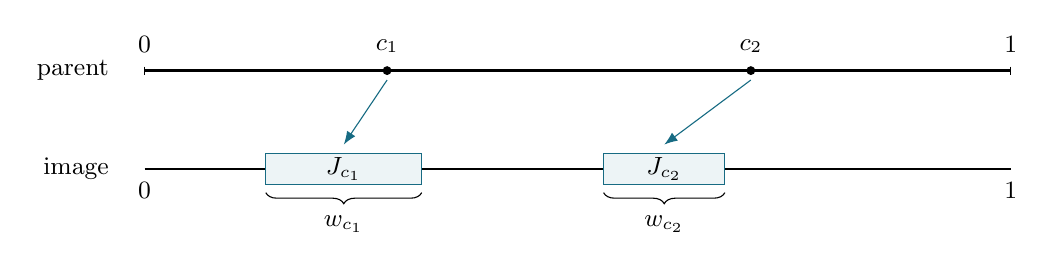
\begin{tikzpicture}[x=11cm,y=1cm,>=Latex,font=\small]
\draw[thick] (0,0)--(1,0);
\node[anchor=east] at (-.03,0) {parent};
\foreach \p/\s in {0/0,.28/{c_1},.7/{c_2},1/1}{
  \draw (\p,.05)--(\p,-.05); \node[above] at (\p,.1) {$\s$};}
\fill (.28,0) circle(1.6pt); \fill (.7,0) circle(1.6pt);
\draw[thick] (0,-1.25)--(1,-1.25);
\node[anchor=east] at (-.03,-1.25) {image};
\filldraw[draw=accent,fill=pale] (.14,-1.45) rectangle (.32,-1.05);
\filldraw[draw=accent,fill=pale] (.53,-1.45) rectangle (.67,-1.05);
\node at (.23,-1.25) {$J_{c_1}$};
\node at (.60,-1.25) {$J_{c_2}$};
\draw[->,accent] (.28,-.12)--(.23,-.94);
\draw[->,accent] (.70,-.12)--(.60,-.94);
\draw[decorate,decoration={brace,mirror,amplitude=4pt}]
  (.14,-1.55)--(.32,-1.55) node[midway,below=5pt] {$w_{c_1}$};
\draw[decorate,decoration={brace,mirror,amplitude=4pt}]
  (.53,-1.55)--(.67,-1.55) node[midway,below=5pt] {$w_{c_2}$};
\node[below] at (0,-1.30) {$0$};
\node[below] at (1,-1.30) {$1$};
\end{tikzpicture}
\caption{The packing map has slope $1/2$ between anchors. Its jump at each
anchor reserves an interval for the entire child subtree. The widths are
shown schematically; their values are given by \eqref{eq:child-weight}.}
\label{fig:packing}
\end{figure}

For a parent--child edge $c$, let $s_c$ be the number of original labels in
the child's entire subtree, and put
\begin{equation}\label{eq:W}
\mathcal W=\prod_{\text{parent--child edges }c}w_c^{s_c}.
\end{equation}
A comparison does not change $\mathcal W$. A refinement into a child of
width $w$ multiplies it by $w$: the refined label crosses that edge, while
its membership in every other subtree remains unchanged. This holds for
both a new child and an existing child.

\Needspace{12\baselineskip}
\begin{lemma}[Packing volume]\label{lem:packing}
The recursive map is injective and preserves the represented order. Its
image $\mathcal I\subseteq(0,1)^n$ has volume
\begin{equation}\label{eq:packed-volume}
\vol(\mathcal I)=2^{-n}Z\mathcal W.
\end{equation}
Consequently, if the transcript determines a unique total order, then
\begin{equation}\label{eq:terminal}
n!Z\mathcal W\le2^n.
\end{equation}
\end{lemma}
\begin{proof}
The map $G$ puts each free position on the correct side of every child
interval. Recursion therefore preserves the order of the original labels.
Anchors and widths are fixed within the state. The image coordinate of a
label depends only on its one free coordinate, through a strictly increasing
map, so the whole map is injective.

Partition the domain at the finitely many anchor hyperplanes. On each piece,
the map of a label is affine. Its slope is $1/2$ at its free coordinate,
multiplied by the widths of the child intervals containing that label along
the path to the root. There are exactly $n$ factors of $1/2$, one per free
coordinate. An edge width $w_c$ occurs $s_c$ times. Thus the Jacobian on
every piece is $2^{-n}\mathcal W$. The domain, a product of the node regions,
has volume $Z$. Injectivity lets us add the image volumes of the pieces,
proving \eqref{eq:packed-volume}.

At completion, legality places the image in the region of the cube realizing
the unique transcript order. The $n!$ coordinate-order regions have equal
volume $1/n!$, since coordinate permutations preserve volume and equality
hyperplanes have volume zero. Hence $2^{-n}Z\mathcal W\le1/n!$.
\end{proof}

\subsection{The addresses of a path}

The same bound on child widths controls a path repair.

\begin{lemma}[Address length of a path batch]\label{lem:path-address}
The $H$ labels of a selected directed path enter distinct children of their
parent. If their address lengths are $m_1,\ldots,m_H$, then
\begin{equation}\label{eq:path-charge}
\sum_{i=1}^H m_i\ge kH.
\end{equation}
\end{lemma}
\begin{proof}
Every arrow on the selected path is an answered comparison. Its labels are
therefore pairwise comparable in the public transcript, and remain so after
arrows are deleted. By Lemma~\ref{lem:admission}, two of these labels cannot
be admitted to the same child. The procedure completes all $H$ refinements
in this parent, so their distinct child widths have sum at most $1/2$.
The arithmetic--geometric mean inequality gives
\[
\prod_{i=1}^H w(m_i)\le(1/(2H))^H.
\]
Substitute \eqref{eq:child-weight} and take logarithms:
\[
(1+1/k)\sum_i m_i\ge H\bigl(\log H-\log(2k)\bigr).
\]
Since $H=2^{2k}$ and $\log(2k)\le k-1$ for integers $k\ge4$, the
right-hand side is at least $(k+1)H$. Division by $1+1/k$ proves the claim.
The auxiliary inequality follows from $2k\le2^{k-1}$, true at $k=4$ and
preserved when $k$ increases by one.
\end{proof}

\section{Why the adversary forces many comparisons}\label{sec:potential}

Recall from Algorithm~\ref{alg:compare} that a larger degree threshold $k$
lets the adversary retain more comparisons involving each item before
moving it into a child. Increasing $k$ lets the adversary force a comparison
count closer to $n\log n$. The following bound quantifies this dependence.

\begin{theorem}[Comparison bound]\label{thm:fixed-stage}
For every power of two $k\ge64$, the adversary of
Algorithm~\ref{alg:compare}, with the remaining parameter choices in
Table~\ref{tab:parameters}, is deterministic and legal, and every call
terminates. Every correct sorter makes at least
\begin{equation}\label{eq:exact-bound}
\frac{n\log n-3n}{1+(2\log k+17)/k}
\end{equation}
comparisons.
\end{theorem}

For this section, fix a power of two $k\ge64$.
Section~\ref{sec:runtime} chooses $k$ as a function of $n$ so that it grows
without bound while the adversary's running time remains polynomial.

The proof uses a random experiment that chooses a node and a position
for each item. At termination, all assignments admitted by the state have
the same relative order, so their probability is at most $1/n!$. We bound
this probability from below using the feasible volumes within nodes and
the probabilities of the child choices made during refinement. Relating
those child choices to the volume gained during refinement will leave
only a small additional loss per comparison.

\subsection{Volume changes}\label{sec:guarantees}

We first measure the freedom left within the individual nodes. At a node
$v$, the feasible assignments form the region
\begin{equation}\label{eq:node-region}
K_v=\{X:a_x<X_x<b_x\text{ for every free }x,
       \quad X_x<X_y\text{ for every in-node arc }x\to y\}.
\end{equation}
Write $V_v=\vol(K_v)$ and take the product over the adversary's tree:
\begin{equation}\label{eq:Z}
Z=\prod_v V_v.
\end{equation}
Each item has a position variable at exactly one node, so the product
region has dimension $n$. A node with no free items contributes volume
one. Initially $Z=1$; whenever every node has positive volume,
$0<Z\le1$.

Choose the estimation error to be
\begin{equation}\label{eq:estimation-error}
\eta=\frac1{100k}.
\end{equation}
By Lemma~\ref{lem:estimation}, each estimated answer retains at least
$1/2-\eta$ of its node's volume. Its decrease in $\log Z$ is therefore
at most
\begin{equation}\label{eq:comparison-loss}
a_\eta=-\log(1/2-\eta)\le1+\frac1{2k}.
\end{equation}
For the inequality, use
$2^{-1/(2k)}\le1-1/(4k)\le1-1/(50k)=1-2\eta$.
An answer already determined by the stored constraints leaves $Z$ unchanged.

Refinement fixes an item's position in its parent and gives it a fresh
unit coordinate in a child. Write
\begin{equation}\label{eq:refinement-gain}
g=\log\frac{Z_{\rm after}}{Z_{\rm before}}
\end{equation}
for the resulting change in $\log Z$. We call $g$ the refinement's
\emph{volume gain}; it can be negative.

The algorithm must preserve positive node volumes and the bounds needed
by the estimator. It must also return answers consistent with the earlier
comparisons. The following proposition gives these guarantees.

\begin{proposition}[Consistency and termination]\label{prop:legality}
With the parameter choices of Theorem~\ref{thm:fixed-stage}, every reached
state has positive node volumes and represents only orders consistent with
the transcript. Every comparison call terminates and performs at most $n$
refinements. Every in-node DAG has degree at most $k$ and directed paths
of fewer than $2H$ vertices throughout the interaction.
\end{proposition}

Section~\ref{sec:repairs} proves Proposition~\ref{prop:legality}.

\subsection{The cost of choosing a child}\label{sec:movement-volume}\label{sec:accounting}

The product $Z$ measures freedom within individual nodes. For example,
two items stored alone in separate children can each retain the full
interval $(0,1)$, giving $Z=1$, even though the child anchors fix their order.
To account for the order determined by the tree, we use a random experiment
on a fixed state.

Start at the root of the adversary's tree. At a visited node, stop with
probability $1/2$. Otherwise, choose an anchor by a walk in the implicit
anchor tree: at each node of that tree, select its position with probability
$1/k$; otherwise, move to the left or right child with equal probability.
If the selected anchor has an existing child in the adversary's tree,
continue the experiment in that child. Otherwise, stop at the current
node. Whenever the experiment stops in the adversary's tree, choose a
uniform coordinate in $(0,1)$ there.

The walk selecting an anchor terminates almost surely. A particular
anchor at depth $m$ requires $m$ specified left or right choices, so an
existing child at that anchor is entered with probability
\begin{equation}\label{eq:child-weight}
w(m)=\frac1{2k}\left(\frac{1-1/k}{2}\right)^m
     =\frac{2^{-\gamma m}}{2k},
\qquad \gamma=1-\log(1-1/k).
\end{equation}
The probability of stopping at each visited node of the adversary's tree
is at least $1/2$. Since the state has a finite tree, the experiment
produces a node and a coordinate almost surely.

Sample one such position independently for each of the $n$ labels.
The tree orders these positions by the same rule as in
Section~\ref{sec:overview}: compare a coordinate with the child anchors,
and order positions inside one child recursively. Ties have probability
zero, and all labels use the same distribution. Permuting the labels
therefore shows that each relative order has probability $1/n!$.

For the counting argument, measure a child choice by its contribution to
the negative logarithm of the probability:
\begin{equation}\label{eq:child-cost}
\ell(m)=-\log w(m)=\gamma m+\log k+1.
\end{equation}
The next lemma expresses the final restriction to one order in terms of
these costs.

\begin{lemma}[Bound at termination]\label{lem:packing}
Suppose the transcript determines a unique total order. If $m_r$ is the
anchor depth used by refinement $r$, then
\begin{equation}\label{eq:terminal}
\log(n!)\le n-\log Z+\sum_r\ell(m_r).
\end{equation}
\end{lemma}
\begin{proof}
Consider the event that every label stops at the node where its record is
stored, and that the sampled coordinates satisfy all the in-node
constraints. Conditional on the chosen stopping nodes, the coordinates
are independent and uniform, so the probability of satisfying the
constraints is $Z$.

The stopping probabilities contribute at least $2^{-n}$. Since records
only move downward, their required paths, counted separately for each
label, contain exactly the edge traversals made by refinements. The child
choices therefore contribute $\prod_r w(m_r)$. The event has probability
at least
\[
Z\,2^{-n}\prod_r w(m_r)=Z\,2^{-n-\sum_r\ell(m_r)}.
\]
By Proposition~\ref{prop:legality}, the event produces an order consistent
with the transcript. The unique such order has probability $1/n!$ in the
random experiment. Comparing these probabilities and taking logarithms
proves \eqref{eq:terminal}.
\end{proof}

\subsection{The guarantees needed from refinement}\label{sec:refinement-cost}

We now compare each child-choice cost with the corresponding volume gain.
The required bounds distinguish the three reasons for moving an item in
Algorithm~\ref{alg:compare}. Choose the path threshold
\begin{equation}\label{eq:path-threshold}
H=2^k.
\end{equation}
Outside a path batch, the algorithm refines a queried item because its
vertex has degree $k$ or its coordinate is narrow. When both hold, count
it as a degree refinement. Set
\begin{equation}\label{eq:charge-coefficient}
\lambda=1+\frac{\log k+10}{k}.
\end{equation}
The following lemma controls the cost of each kind of refinement using
its volume gain. Degree refinements receive an additional allowance.

\begin{lemma}[Cost of refinement]\label{lem:refinement-cost}
A degree refinement with anchor depth $m$ and volume gain $g$ satisfies
\[
\ell(m)\le\lambda g+\log k+6.
\]
A narrow refinement satisfies $\ell(m)\le\lambda g$.
For a complete path batch with depths $m_i$ and gains $g_i$,
\[
\sum_{i=1}^H\ell(m_i)\le\lambda\sum_{i=1}^H g_i.
\]
\end{lemma}

Section~\ref{sec:refinement-guarantee} proves this lemma. Narrow refinements
supply a large individual gain, and complete path batches supply a large
average gain. These gains cover their child-choice costs. Degree
refinements may need the extra allowance, which we charge to earlier
comparisons in the proof below.

\subsection{The comparison bound}\label{sec:comparison-cost}

\begin{proof}[Proof of Theorem~\ref{thm:fixed-stage}]
Proposition~\ref{prop:legality} gives consistency and termination of every
call. The procedures and their tie rules are deterministic.
Suppose the sorter finishes after $q$ comparisons, and write $j=\log k$.
Correctness requires its terminating transcript to determine a unique
total order, so Lemma~\ref{lem:packing} applies.

There are at most $q/k$ degree refinements: each deletes $k$ in-node arcs,
each comparison inserts at most one arc, and an inserted arc can be deleted
only once. Apply Lemma~\ref{lem:refinement-cost} to these refinements, the
remaining individual refinements, and the complete path batches. This gives
\begin{equation}\label{eq:refinement-total}
\sum_r\ell(m_r)\le\lambda\sum_r g_r+\frac{j+6}{k}\,q.
\end{equation}
Each comparison decreases $\log Z$ by at most $a_\eta$, while a refinement
changes it by $g_r$. Since initially $Z=1$,
\[
\sum_r g_r\le\log Z+a_\eta q.
\]
Substitute this into \eqref{eq:refinement-total} and then into the terminal
bound \eqref{eq:terminal}:
\begin{equation}\label{eq:comparison-total}
\log(n!)\le n+(\lambda-1)\log Z
              +\left(\lambda a_\eta+\frac{j+6}{k}\right)q.
\end{equation}
The term $(\lambda-1)\log Z$ is nonpositive. Moreover,
\begin{align}
\lambda a_\eta+\frac{j+6}{k}
&\le1+\frac{2j+33/2}{k}+\frac{j+10}{2k^2}\nonumber\\
&\le1+\frac{2j+17}{k},\label{eq:comparison-charge}
\end{align}
where the last inequality uses $j+10\le k$.
Finally,
\[
\log(n!)\ge\int_1^n\log x\,dx
=n\log n-\frac{n}{\ln2}+\frac1{\ln2}.
\]
Combining this estimate with \eqref{eq:comparison-total},
\eqref{eq:comparison-charge}, and $1+1/\ln2<3$ proves
\eqref{eq:exact-bound}.
\end{proof}

The next section proves the refinement and consistency guarantees used above.

\section{A uniform polynomial-time implementation}\label{sec:runtime}

For each fixed degree threshold $k$, the preceding sections give a
finite deterministic algorithm. Its local calculations depend on $k$,
while its interval endpoints depend on the comparison history. We first
bound the size of the maintained state, then choose $k$ slowly
enough that the local calculations also take polynomial time.
Computation is measured on a fixed deterministic multitape Turing machine,
with integers represented in binary.

\subsection{Bounding the state throughout the interaction}

The first test in Algorithm~\ref{alg:compare} answers any comparison
already implied by the global comparison DAG. Such a call leaves the
stored state unchanged. Every other call starts with an incomparable pair
and makes that pair comparable permanently. Thus at most $\binom n2$
calls can change the state, however often the sorter repeats a comparison.

Lemmas~\ref{lem:preparation} and~\ref{lem:restoration} bound the number of
refinements in one call by $n+2$. Consequently the total number $P$ of
refinements, including those in a call still in progress, satisfies
\begin{equation}\label{eq:refinement-runtime}
P\le(n+2)\binom n2.
\end{equation}
Each refinement creates at most one node in the adversary's tree, so
that tree has at most $P+1$ nodes. The global comparison DAG has $n$
vertices and at most $\binom n2$ arcs. The transcript is the output stream;
its order constraints are retained in this DAG.

We store an anchor by its path in the implicit anchor tree. A path of
length $m$ gives its interval and position by $m$ halvings of $[0,1]$;
the position has $m+1$ fractional binary digits. Anchor comparisons use
these exact numerical positions.

For a wide item, Lemma~\ref{lem:median-search} bounds both the number of
search tests and the anchor precision by
\[
K_0(k)=\ceil{\log(4(B+1)R)}+2.
\]
For a narrow item, suppose the current endpoints have at most $\Lambda$
fractional digits. Its positive effective width is at least $2^{-\Lambda}$.
The selected anchor-tree interval has length $2^{-m}>W_x/8$, so
$m<\Lambda+3$. The new anchor therefore has at most $\Lambda+3$ fractional
digits. Tightening takes maxima and minima of endpoints and adds no digits.
After $P$ refinements,
\begin{equation}\label{eq:precision}
\Lambda\le K_0(k)+3P.
\end{equation}
The narrow walk makes at most $\Lambda+2$ steps, using integers with
$O(\Lambda)$ bits at each step.

\subsection{Choosing the degree threshold}\label{sec:parameter-selection}

Lemma~\ref{lem:exact-local-volume} bounds a local volume calculation by
$C_0(b)(\Lambda+1)^2$ bit operations, where the number $b$ of retained
coordinates depends only on $k$. The function $C_0$ is computable from
the finite enumeration in its proof. Finding the neighborhood and its
effective endpoints uses graph operations on at most $n$ vertices, with
a fixed polynomial cost in $n$ and $\Lambda$.

Choose a computable integer $C(k)$ that bounds $K_0(k)$ and all
parameter-dependent factors in one local calculation, including
$C_0(b)$. For powers of two $k=64,128,\ldots$, a fixed program writes the
complete parameter tuple and $C(k)$ in binary. On input size $n$, simulate
this program for $n$ steps. Among the tuples it has completed, choose the
largest $k$ satisfying
\begin{equation}\label{eq:stage-gate}
C(k)\le n.
\end{equation}
Use these parameters for the entire interaction. If no tuple qualifies,
answer all comparisons according to the fixed label order.

The initialization is polynomial: the simulation writes at most $n$
bits, and its completed tuples can be parsed and compared within a
polynomial bound. For every fixed $k$, the tuple is written in some finite
time $T(k)$. Once $n\ge\max\{T(k),C(k)\}$, it is available and affordable.
Hence the chosen $k(n)$ tends to infinity.

For a selected tuple, \eqref{eq:refinement-runtime}--\eqref{eq:stage-gate}
give $\Lambda=O(n^3)$ and a polynomial number of stored nodes. Every local
volume calculation has a fixed polynomial bit cost. A comparison call
makes at most $n+2$ refinements, and each wide refinement uses at most
$K_0(k)\le n$ estimates. Narrow refinements use the bounded walks described
above. Routing queries, propagating bounds, and testing reachability take
polynomial time in the stored state. Directed-path lengths are computed
in reverse topological order; if $H>n$, no path can require repair.
All tie rules can be implemented by scanning labels in order. Thus each
comparison is answered within one fixed polynomial number of bit
operations, independent of the chosen parameter and of the length of
the preceding interaction.

\begin{proof}[Proof of Theorem~\ref{thm:main}]
Initialization and every comparison call are deterministic and take
polynomial time. For all sufficiently large $n$, a parameter tuple
qualifies. Theorem~\ref{thm:fixed-stage} gives legality and forces
\[
q\ge\frac{n\log n-3n}{1+(2\log k(n)+18)/k(n)}
=(1-o(1))n\log n,
\]
since $k(n)\to\infty$. The fixed-order rule for the remaining input sizes
is also deterministic and legal.
\end{proof}

\appendix
\section{Coordinate densities}\label{app:geometry}

We prove the density bounds used to choose anchors and to turn coordinate
approximation into probability approximation. The first bounds follow by
fixing the incomparable coordinates and comparing sections of the remaining
convex region. Let $V$ be the set of coordinates, let $N=|V|$, and let
$K\subseteq\R^V$ be their feasible region.
For a coordinate $x$ and a real number $t$, write
\[
K_x(t)=\{(z_i)_{i\ne x}:z\in K,\ z_x=t\},
\qquad S_x(t)=\vol_{N-1}K_x(t).
\]
Here $K_x(t)$ is the $(N-1)$-dimensional section obtained by fixing
coordinate $x$ at $t$. The uniform distribution on $K$
therefore gives $x$ the density
\[
f_x(t)=\frac{S_x(t)}{\vol_N K}.
\]
These formulas define $f_x$ pointwise, and we use this definition throughout.
If some coordinates have already been fixed, we use the same
definitions in the remaining free coordinates. In dimension zero, the
volume of the singleton consisting of the empty assignment is one.

\begin{proof}[Proof of Lemma~\ref{lem:fiber}]
We may first fix any prescribed set of coordinates incomparable with $x$,
at values leaving a positive-volume slice; write $f_x$ for its coordinate
density. Fixing a coordinate turns its incident inequalities
into interval bounds. These bounds propagate along directed paths, so
fixing an incomparable coordinate leaves $x$'s effective endpoints
unchanged. By Lemma~\ref{lem:interior}, its projection interval remains
$(\ell,r)$. The same argument applies successively as more incomparable
coordinates are fixed.

Now fix all the remaining coordinates incomparable with $x$. For each
choice leaving a nonempty slice, the remaining feasible region $C$ is
open and convex, has dimension $d\le B+1$, and projects onto $(\ell,r)$
in coordinate $x$. Write $S(t)$ for its section volume at $x=t$ and
$g(t)=S(t)/\vol C$ for the resulting density.

Choose points in $\overline C$ whose $x$-coordinates are $\ell$ and $r$.
Such points exist because $C$ is bounded. For $\ell<t<s<r$, join every
point of the section at $t$ to the point at $r$. Since $C$ is open and
convex, the image at $x=s$ lies in the section of $C$ there. Each of its
$d-1$ directions is scaled by $(r-s)/(r-t)$, so
\begin{equation}\label{eq:push-upper}
S(s)\ge\left(\frac{r-s}{r-t}\right)^{d-1}S(t)
\qquad(t<s).
\end{equation}
Joining instead to the point at $\ell$ gives
\begin{equation}\label{eq:push-lower}
S(s)\ge\left(\frac{s-\ell}{t-\ell}\right)^{d-1}S(t)
\qquad(s<t).
\end{equation}
Normalize these inequalities and integrate over $s$ on both sides of $t$:
\[
1\ge g(t)\left(
\int_\ell^t\left(\frac{s-\ell}{t-\ell}\right)^{d-1}ds+
\int_t^r\left(\frac{r-s}{r-t}\right)^{d-1}ds\right)
=\frac{Wg(t)}{d}.
\]
Thus $g(t)\le d/W\le(B+1)/W$.

For the lower bound, choose $t_0$ with $g(t_0)\ge1/W$, which exists
because $g$ integrates to one over an interval of length $W$. For any
$s\in[\ell+W/4,r-W/4]$, the appropriate ratio in
\eqref{eq:push-upper} or \eqref{eq:push-lower} is at least $1/4$.
Consequently
\[
g(s)\ge4^{-(d-1)}g(t_0)\ge\frac{4^{-B}}{W}.
\]
The case $s=t_0$ satisfies the same bound directly.

Finally, average over the additional incomparable coordinates fixed in
the second paragraph. If $\omega$ denotes their values, $C_\omega$ the
remaining region, and $g_\omega$ its coordinate density, integration of
each section gives the pointwise identity
\[
f_x(t)=
\frac{\int \vol(C_\omega)g_\omega(t)\,d\omega}
     {\int \vol(C_\omega)\,d\omega}.
\]
Empty slices contribute zero. The bounds on $g_\omega$ are uniform in
$\omega$, so they hold for $f_x$ at every $t$. This proves both the
unconditional bounds and the bounds after the initial conditioning.
\end{proof}

The coordinate densities above are log-concave pointwise: the uniform
density on $K$ is log-concave, and integrating out the other coordinates
preserves this property by Pr\'ekopa's marginal theorem
\cite[Theorem~8]{prekopa}. We finish with the density bound used for
positions having substantial probability on each side.

\begin{proof}[Proof of Lemma~\ref{lem:central-quantiles}]
For $s\le c\le t$, log-concavity gives
\[
f(s)f(t)\le f(c)f(s+t-c).
\]
Indeed, $c$ and $s+t-c$ are complementary convex combinations of $s,t$;
multiply the two log-concavity inequalities. Fixing $t\ge c$ and
integrating over $s\le c$ gives
\[
p f(t)\le f(c)\int_{-\infty}^c f(s+t-c)\,ds\le f(c).
\]
Here the first inequality uses the mass at least $p$ to the left of $c$,
and the last uses that a density integrates to one. Fixing $s\le c$ and
integrating over $t\ge c$ instead uses the right-hand mass and gives
$p f(s)\le f(c)$. Taking the supremum over both sides of $c$ proves the
claim.
\end{proof}

\clearpage
\begin{thebibliography}{10}

\bibitem{knuth}
Donald E. Knuth.
\emph{The Art of Computer Programming, Volume 3: Sorting and Searching.}
Second edition, Addison-Wesley, 1998.
\href{https://www.informit.com/store/art-of-computer-programming-volume-3-sorting-and-searching-9780201896855}{Publisher's page}.

\bibitem{fredman}
Michael L. Fredman.
\emph{How good is the information theory bound in sorting?}
Theoretical Computer Science 1(4), 355--361, 1976.
\href{https://doi.org/10.1016/0304-3975(76)90078-5}{doi:10.1016/0304-3975(76)90078-5}.

\bibitem{atallah}
Mikhail J. Atallah and S. Rao Kosaraju.
\emph{An adversary-based lower bound for sorting.}
Information Processing Letters 13(2), 55--57, 1981.

\bibitem{borodin}
Allan Borodin, Leonidas J. Guibas, Nancy A. Lynch, and Andrew C. Yao.
\emph{Efficient searching using partial ordering.}
Information Processing Letters 12(2), 71--75, 1981.
\href{https://doi.org/10.1016/0020-0190(81)90005-3}{doi:10.1016/0020-0190(81)90005-3}.

\bibitem{richards}
Dana Richards and Pravin M. Vaidya.
\emph{On the distribution of comparisons in sorting algorithms.}
BIT 28, 764--774, 1988.
\href{https://lic225.github.io/vaidya/sorting_BIT88.pdf}{Authors' paper}.

\bibitem{brodal}
Gerth St{\o}lting Brodal, Shiva Chaudhuri, and Jaikumar Radhakrishnan.
\emph{The randomized complexity of maintaining the minimum.}
Nordic Journal of Computing 3(4), 337--351, 1996.
\href{https://www.brics.dk/RS/96/40/BRICS-RS-96-40.pdf}{Authors' report, BRICS RS-96-40}.


\bibitem{kzz-min}
Haim Kaplan, Or Zamir, and Uri Zwick.
\emph{The amortized cost of finding the minimum.}
Proceedings of the Twenty-Sixth Annual ACM--SIAM Symposium on Discrete Algorithms
(SODA), 757--768, 2015. Published online 22 December 2014.
\href{https://doi.org/10.1137/1.9781611973730.51}{doi:10.1137/1.9781611973730.51}.
\href{https://zamir.prof/pub/FindMin_OrZamir.pdf}{Authors' paper}.

\bibitem{kzz}
Haim Kaplan, Or Zamir, and Uri Zwick.
\emph{A sort of an adversary.}
Proceedings of the Thirtieth Annual ACM--SIAM Symposium on Discrete Algorithms
(SODA), 1291--1310, 2019.
\href{https://doi.org/10.1137/1.9781611975482.79}{doi:10.1137/1.9781611975482.79}.

\bibitem{stanley}
Richard P. Stanley.
\emph{Two poset polytopes.}
Discrete \& Computational Geometry 1, 9--23, 1986.
\href{https://doi.org/10.1007/BF02187680}{doi:10.1007/BF02187680}.
\href{https://math.mit.edu/~rstan/pubs/pubfiles/66.pdf}{Author's copy}.

\bibitem{brightwell}
Graham Brightwell and Peter Winkler.
\emph{Counting linear extensions.}
Order 8(3), 225--242, 1991.
\href{https://doi.org/10.1007/BF00383444}{doi:10.1007/BF00383444}.

\bibitem{dfk}
Martin Dyer, Alan Frieze, and Ravi Kannan.
\emph{A random polynomial-time algorithm for approximating the volume of convex bodies.}
Journal of the ACM 38(1), 1--17, 1991.
\href{https://doi.org/10.1145/102782.102783}{doi:10.1145/102782.102783}.
\href{https://www.math.cmu.edu/~af1p/Texfiles/oldvolume.pdf}{Authors' manuscript}.

\bibitem{kahn-kim}
Jeff Kahn and Jeong Han Kim.
\emph{Entropy and sorting.}
Journal of Computer and System Sciences 51(3), 390--399, 1995.
\href{https://doi.org/10.1006/jcss.1995.1077}{doi:10.1006/jcss.1995.1077}.


\bibitem{prekopa}
Andr\'as Pr\'ekopa.
\emph{On logarithmic concave measures and functions.}
Acta Scientiarum Mathematicarum 34, 335--343, 1973.
\href{https://acta.bibl.u-szeged.hu/14411/1/math_034_335-343.pdf}{Publisher's paper}.

\bibitem{cardinal-production}
Jean Cardinal, Samuel Fiorini, Gwena\"el Joret, Rapha\"el M. Jungers,
and J. Ian Munro.
\emph{An efficient algorithm for partial order production.}
SIAM Journal on Computing 39(7), 2927--2940, 2010.
\href{https://doi.org/10.1137/090759860}{doi:10.1137/090759860}.
\href{https://arxiv.org/abs/0811.2572}{Authors' manuscript}.

\bibitem{imprecise-points}
Ivor van der Hoog, Irina Kostitsyna, Maarten L\"offler, and Bettina Speckmann.
\emph{Preprocessing ambiguous imprecise points.}
35th International Symposium on Computational Geometry (SoCG),
LIPIcs 129, 42:1--42:16, 2019.
\href{https://doi.org/10.4230/LIPIcs.SoCG.2019.42}{doi:10.4230/LIPIcs.SoCG.2019.42}.

\bibitem{interval-orders}
Ivor van der Hoog, Irina Kostitsyna, Maarten L\"offler, and Bettina Speckmann.
\emph{Sorting under partial (interval order) information.}
Journal of Computational Geometry 15(1), 143--171, 2024.
\href{https://doi.org/10.20382/jocg.v15i1a6}{doi:10.20382/jocg.v15i1a6}.


\bibitem{marked-order-polytopes}
Federico Ardila, Thomas Bliem, and Dido Salazar.
\emph{Gelfand--Tsetlin polytopes and Feigin--Fourier--Littelmann--Vinberg
polytopes as marked poset polytopes.}
Journal of Combinatorial Theory, Series A 118(8), 2454--2462, 2011.
\href{https://doi.org/10.1016/j.jcta.2011.06.004}{doi:10.1016/j.jcta.2011.06.004}.
\href{https://arxiv.org/abs/1008.2365}{arXiv:1008.2365}.

\bibitem{bencs-regts-volume}
Ferenc Bencs and Guus Regts.
\emph{Approximating the volume of a truncated relaxation of the independence polytope.}
Discrete \& Computational Geometry 76, 508--525, 2026.
\href{https://doi.org/10.1007/s00454-026-00824-y}{doi:10.1007/s00454-026-00824-y}.

\bibitem{chan-pak-survey}
Swee Hong Chan and Igor Pak.
\emph{Linear extensions of finite posets.}
EMS Surveys in Mathematical Sciences, published online 17 March 2025.
\href{https://doi.org/10.4171/EMSS/97}{doi:10.4171/EMSS/97}.
\href{https://www.math.ucla.edu/~pak/papers/LEsurvey11.pdf}{Authors' manuscript}.

\bibitem{talvitie-counting}
Topi Talvitie, Kustaa Kangas, Teppo Niinim\"aki, and Mikko Koivisto.
\emph{A scalable scheme for counting linear extensions.}
Proceedings of the Twenty-Seventh International Joint Conference on
Artificial Intelligence (IJCAI), 5119--5125, 2018.
\href{https://www.ijcai.org/proceedings/2018/710}{Publisher's page}.
\href{https://ijcai.org/proceedings/2018/0710.pdf}{Authors' paper}.

\bibitem{haeupler-sorting}
Bernhard Haeupler, Richard Hlad\'ik, John Iacono, V\'aclav Rozho\v{n},
Robert E. Tarjan, and Jakub T\v{e}tek.
\emph{Fast and simple sorting using partial information.}
Proceedings of the Thirty-Sixth Annual ACM--SIAM Symposium on Discrete
Algorithms (SODA), 2025.
\href{https://doi.org/10.1137/1.9781611978322.134}{doi:10.1137/1.9781611978322.134}.
\href{https://arxiv.org/abs/2404.04552}{Authors' manuscript}.

\bibitem{rutschmann-sorting}
Daniel Rutschmann.
\emph{Sorting under partial information with optimal preprocessing time
via unified bound heaps.}
Preprint, 2026. To appear at FOCS 2026.
\href{https://arxiv.org/abs/2604.12653}{arXiv:2604.12653}.

\bibitem{huber-sampling}
Mark Huber.
\emph{Near-linear time simulation of linear extensions of a height-2
poset with bounded interaction.}
Chicago Journal of Theoretical Computer Science 2014, Article 3, 1--16.
\href{https://doi.org/10.4086/cjtcs.2014.003}{doi:10.4086/cjtcs.2014.003}.

\bibitem{propp-wilson}
James G. Propp and David B. Wilson.
\emph{Exact sampling with coupled Markov chains and applications to
statistical mechanics.}
Random Structures \& Algorithms 9(1--2), 223--252, 1996.
\href{https://www.stat.berkeley.edu/~aldous/206-RWG/RWGpapers/propp_wilson.pdf}{Authors' paper}.

\end{thebibliography}

\end{document}
